
\subsection{Patch Match}

Given an input image $A$ made of overlapping $N\times N$ patches $\{\ti\}$, we want to find the closest patches $\{\si\}$ in an image $B$, i.e.
\begin{equation}
	\si^{*} = \argmin_{\si \in B} d(\ti, \si)
\end{equation}
for some distance $d(\cdot)$, usually the sum of squared differences or a L2 norm.

A naive brute-force computation would enumerate all possible patch assignments and find the best one.
However, this is computationally unreasonnable given the context of our large high resolution image database.

Patch Match~\cite{Barnes09} is a fast approximate nearest neighbor algorithm specifically tuned for image patches and thus our problem.
It is based on the \emph{coherence assumption}, namely that, while patches mapped from $A$ to $B$ can be mapped everywhere in $B$, nearby patches in $A$ are usually mapped together in $B$.

\begin{figure}[ht]
\centering
	\begin{subfigure}[t]{0.155\textwidth}
		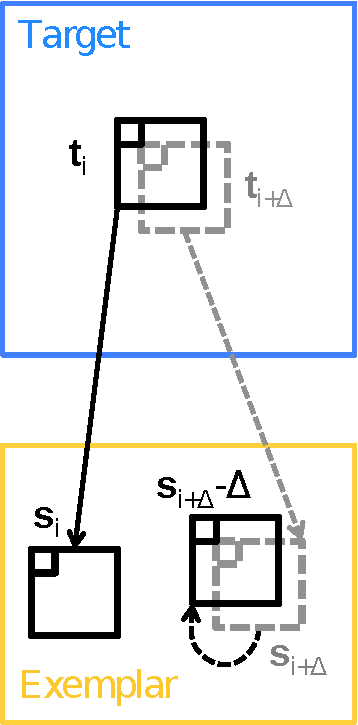
\includegraphics[width=\textwidth]{figures/propagation_text2}
		\caption{Propagation}
	\end{subfigure}
	\begin{subfigure}[t]{0.155\textwidth}
		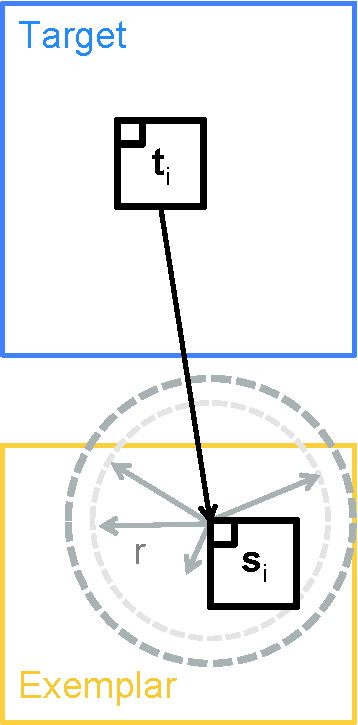
\includegraphics[width=\textwidth]{figures/randsearch_text}
		\caption{Random search}
	\end{subfigure}
	\begin{subfigure}[t]{0.155\textwidth}
		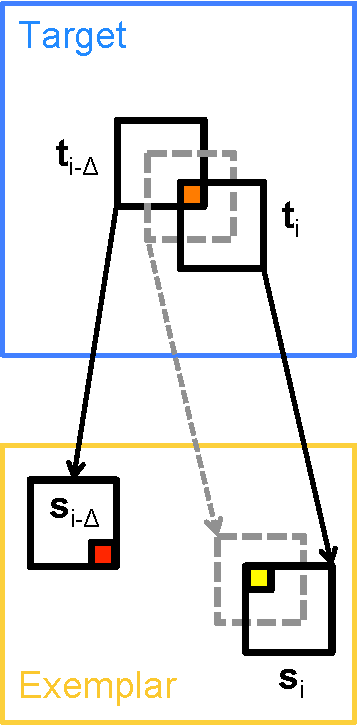
\includegraphics[width=\textwidth]{figures/voting_text}
		\caption{Voting}
	\end{subfigure}
   \caption{The main components of texture synthesis using Patch Match.}
\label{fig:texsynth_patchmatch}
\end{figure}

The algorithm proceeds in scanline-order from an initial guess of the nearest neighbor assignments $\{\ti \to \si\}$ and tries new candidate nearest neighbor patches using two main operations:
\textbf{propagation} which tries to propagate the result of neighboring mappings, and 
\textbf{random search} that randomly samples patches in an exponentially decreasing window (see illustrations in Figure~\ref{fig:texsynth_patchmatch}).

Given these patch assignments, we can transfer localized data.
This last step involves different strategies which we details in Section~\ref{sec:transfer}. 
All of them are forms of \emph{voting} since by having $N\times N$ patches, each of the pixels of our output image technically has as many overlapping patches to choose from.
The usual voting consist of averaging the overlapping pixels which minimizes the average L2 distance.

\paragraph{Extensions}
The Patch Match algorithm has been extended in several ways \cite{Barnes10} including the sampling of rotations, scales and mirrored patch spaces, the use of gain and bias adjustment, a $k$-NN version of the algorithm as well as extra operations (uniform sampling, enrichment and binning).

Application-specific variants of voting have been explored such as Meanshift \cite{Wexler07}, Histogram weighting \cite{Kopf07} as well as Bidirectional Similarity \cite{Simakov08}.